\section{电子在中心势场中的运动}

\begin{quotation}
``在经典力学的基础上,人类征服了太空;\\
在量子力学的基础上,原子世界的面纱已被揭开。''
\end{quotation}

\subsection{经典情形}

根据牛顿力学,粒子在中心力场中必作平面运动;

\index{Spherical potential: 中心力场}

角动量:$\mathord{\buildrel{\lower3pt\hbox{$\scriptscriptstyle\rightharpoonup$}}
\over L}  = \mathord{\buildrel{\lower3pt\hbox{$\scriptscriptstyle\rightharpoonup$}}
\over r}  \times \mathord{\buildrel{\lower3pt\hbox{$\scriptscriptstyle\rightharpoonup$}}
\over p} $;

$\frac{{d\mathord{\buildrel{\lower3pt\hbox{$\scriptscriptstyle\rightharpoonup$}}
\over L} }}{{dt}} = \frac{{d\mathord{\buildrel{\lower3pt\hbox{$\scriptscriptstyle\rightharpoonup$}}
\over r} }}{{dt}} \times \mathord{\buildrel{\lower3pt\hbox{$\scriptscriptstyle\rightharpoonup$}}
\over p}  + \mathord{\buildrel{\lower3pt\hbox{$\scriptscriptstyle\rightharpoonup$}}
\over r}  \times \frac{{d\mathord{\buildrel{\lower3pt\hbox{$\scriptscriptstyle\rightharpoonup$}}
\over p} }}{{dt}}$,
$\mathord{\buildrel{\lower3pt\hbox{$\scriptscriptstyle\rightharpoonup$}}
\over p}  = m\mathord{\buildrel{\lower3pt\hbox{$\scriptscriptstyle\rightharpoonup$}}
\over v} $,
$\mathord{\buildrel{\lower3pt\hbox{$\scriptscriptstyle\rightharpoonup$}}
\over v}  = \frac{{d\mathord{\buildrel{\lower3pt\hbox{$\scriptscriptstyle\rightharpoonup$}}
\over r} }}{{dt}}$,
$\mathord{\buildrel{\lower3pt\hbox{$\scriptscriptstyle\rightharpoonup$}}
\over F}  = m\frac{{d\mathord{\buildrel{\lower3pt\hbox{$\scriptscriptstyle\rightharpoonup$}}
\over v} }}{{dt}}$


$\frac{{d\mathord{\buildrel{\lower3pt\hbox{$\scriptscriptstyle\rightharpoonup$}}
\over L} }}{{dt}} = \mathord{\buildrel{\lower3pt\hbox{$\scriptscriptstyle\rightharpoonup$}}
\over v}  \times m\mathord{\buildrel{\lower3pt\hbox{$\scriptscriptstyle\rightharpoonup$}}
\over v}  + \mathord{\buildrel{\lower3pt\hbox{$\scriptscriptstyle\rightharpoonup$}}
\over r}  \times m\frac{{d\mathord{\buildrel{\lower3pt\hbox{$\scriptscriptstyle\rightharpoonup$}}
\over v} }}{{dt}} = 0 + \mathord{\buildrel{\lower3pt\hbox{$\scriptscriptstyle\rightharpoonup$}}
\over r}  \times \mathord{\buildrel{\lower3pt\hbox{$\scriptscriptstyle\rightharpoonup$}}
\over F} $

中心势场中,中心力可表示为:$\mathord{\buildrel{\lower3pt\hbox{$\scriptscriptstyle\rightharpoonup$}}
\over F}  = F(r)\mathord{\buildrel{\lower3pt\hbox{$\scriptscriptstyle\rightharpoonup$}}
\over e} _r $; (库仑力:$\mathord{\buildrel{\lower3pt\hbox{$\scriptscriptstyle\rightharpoonup$}}
\over F}  = \frac{1}{{4\pi \varepsilon _0 }}\frac{{Z_1 Z_2 e^2 }}{{r^2 }}\mathord{\buildrel{\lower3pt\hbox{$\scriptscriptstyle\rightharpoonup$}}
\over e} _r $)

\index{Coulomb force: 库仑力}

$\frac{{d\mathord{\buildrel{\lower3pt\hbox{$\scriptscriptstyle\rightharpoonup$}}
\over L} }}{{dt}} = \mathord{\buildrel{\lower3pt\hbox{$\scriptscriptstyle\rightharpoonup$}}
\over r}  \times F(r)\mathord{\buildrel{\lower3pt\hbox{$\scriptscriptstyle\rightharpoonup$}}
\over e} _r  = 0$;
即角动量守恒:$\mathord{\buildrel{\lower3pt\hbox{$\scriptscriptstyle\rightharpoonup$}}
\over L}  = m\mathord{\buildrel{\lower3pt\hbox{$\scriptscriptstyle\rightharpoonup$}}
\over r}  \times \mathord{\buildrel{\lower3pt\hbox{$\scriptscriptstyle\rightharpoonup$}}
\over v}  = mr^2 \dot \theta \mathord{\buildrel{\lower3pt\hbox{$\scriptscriptstyle\rightharpoonup$}}
\over e} _k $

所以在中心势场下,粒子必作平面运动(与常矢量$\vec L$垂直的平面),可以取平面极坐标($r,\theta $)研究粒子的运动;

拉格朗日函数:$L = T - V = \frac{1}{2}m\left( {\dot r^2  + r^2 \dot \theta ^2 } \right) - V(r)$

粒子角动量:$p_\theta   = \frac{{\partial L}}{{\partial \dot \theta }} = mr^2 \dot \theta $

关于$\theta $的运动方程:$\frac{d}{{dt}}\frac{{\partial L}}{{\partial \dot \theta }} - \frac{{\partial L}}{{\partial \theta }} = 0$,$\frac{d}{{dt}}mr^2 \dot \theta  = \frac{{\partial L}}{{\partial \theta }} = 0$

即角动量守恒:$mr^2 \dot \theta  = l$,

关于$r$的运动方程:$\frac{d}{{dt}}\frac{{\partial L}}{{\partial \dot r}} - \frac{{\partial L}}{{\partial r}} = 0$,$p_r  = \frac{{\partial L}}{{\partial \dot r}} = m\dot r$

$\frac{d}{{dt}}\left( {m\dot r} \right) - \left( {mr\dot \theta ^2  - \frac{{\partial V}}{{\partial r}}} \right) = 0$, 定义中心势对应的力:$F(r) =  - \frac{{\partial V}}{{\partial r}}$


$m\ddot r - mr\dot \theta ^2  = F(r)$,由角动量守恒:$m\ddot r - \frac{{l^2 }}{{mr^3 }} = F(r)$

这样就把问题化为单变量问题,仅与$r$有关;

能量守恒:$E = T + V = \frac{1}{2}m\left( {\dot r^2  + r^2 \dot \theta ^2 } \right) + V(r) = \frac{1}{2}m\dot r^2  + \frac{{l^2 }}{{2mr^2 }} + V(r)$

利用:$m\ddot r \cdot \dot r = \frac{d}{{dt}}\left( {\frac{1}{2}m\dot r^2 } \right) =  - \frac{{dr}}{{dt}}\frac{d}{{dr}}\left( {V + \frac{{l^2 }}{{2mr^2 }}} \right) =  - \frac{d}{{dt}}\left( {V + \frac{{l^2 }}{{2mr^2 }}} \right)$

可以证明:$m\ddot r = F(r) + \frac{{l^2 }}{{mr^3 }} =  - \frac{d}{{dr}}\left( {V + \frac{{l^2 }}{{2mr^2 }}} \right)$

即:$\frac{d}{{dt}}\left( {\frac{1}{2}m\dot r^2  + \frac{{l^2 }}{{2mr^2 }} + V} \right) = 0$
$ \Rightarrow $
$E = \frac{1}{2}m\dot r^2  + \frac{{l^2 }}{{2mr^2 }} + V = {\rm{Const}}$

由能量守恒表达式:$\dot r = \sqrt {\frac{2}{m}\left( {E - V - \frac{{l^2 }}{{2mr^2 }}} \right)} $

即:$dt = \frac{{dr}}{{\sqrt {\frac{2}{m}\left( {E - V - \frac{{l^2 }}{{2mr^2 }}} \right)} }}$,两边积分:从$t = 0$,$r = r_0 $,到$t,r$:


$t = \int_{r_0 }^r {\frac{{dr}}{{\sqrt {\frac{2}{m}\left( {E - V - \frac{{l^2 }}{{2mr^2 }}} \right)} }}} $,积分可解出粒子的轨道方程:$r = r(t)$

轨道方程一般表示为$r = r(\theta )$;

由角动量守恒:$mr^2 \dot \theta  = l$,$d\theta  = \frac{{ldt}}{{mr^2 }}$

所以:$d\theta  = \frac{l}{{mr^2 }}dt = \frac{{ldr}}{{r^2 \sqrt {2m\left( {E - V} \right) - \frac{{l^2 }}{{r^2 }}} }}$;$\theta  = \int {d\theta }  = \int {\frac{{ldr}}{{r^2 \sqrt {2m\left( {E - V} \right) - \frac{{l^2 }}{{r^2 }}} }}} $

$\theta  = \int_{\theta _0 }^\theta  {d\theta }  = \int_{r_0 }^r {\frac{{dr}}{{\frac{{r^2 }}{{l^2 }}\sqrt {2m\left( {E - V} \right) - \frac{{l^2 }}{{r^2 }}} }}}  = \int_{r_0 }^r {\frac{{dr}}{{r^2 \sqrt {\frac{{2mE}}{{l^2 }} - \frac{{2mV}}{{l^2 }} - \frac{1}{{r^2 }}} }}} $


变量变换:$u = \frac{1}{r}$;$du =  - r^{ - 2} dr$;$\theta  - \theta _0  =  - \int_{u_0 }^u {\frac{{du}}{{\sqrt {\frac{{2mE}}{{l^2 }} - \frac{{2mV}}{{l^2 }} - u^2 } }}} $

设:$V(r) =  - \frac{Z}{r}$(库仑势);$\theta  = \theta _0  - \int_{u_0 }^u {\frac{{du}}{{\sqrt {\frac{{2mE}}{{l^2 }} + \frac{{2mZu}}{{l^2 }} - u^2 } }}} $

利用积分关系:$\int {\frac{{dx}}{{\sqrt {\alpha  + \beta x + \gamma x^2 } }} = \frac{1}{{\sqrt { - \gamma } }}} \arccos \left( { - \frac{{\beta  + 2\gamma x}}{{\sqrt {\beta ^2  - 4\alpha \gamma } }}} \right)$

这里:$\alpha  = \frac{{2mE}}{{l^2 }},\beta  = \frac{{2mZ}}{{l^2 }},\gamma  =  - 1,\beta ^2  - 4\alpha \gamma  = \left( {\frac{{2mZ}}{{l^2 }}} \right)^2 \left( {1 + \frac{{2El^2 }}{{mZ^2 }}} \right)$

所以:$\theta  = \theta _0  - \arccos \frac{{\frac{{l^2 u}}{{mZ}} - 1}}{{\sqrt {1 + \frac{{2El^2 }}{{mZ^2 }}} }}$,$\frac{{l^2 u}}{{mZ}} = 1 + \sqrt {1 + \frac{{2El^2 }}{{mZ^2 }}} \cos \left( {\theta  - \theta _0 } \right)$

$\frac{1}{r} = \frac{{mZ}}{{l^2 }}\left( {1 + \sqrt {1 + \frac{{2El^2 }}{{mZ^2 }}} \cos \left( {\theta  - \theta _0 } \right)} \right) = \frac{{1 + e\cos \theta }}{p}$,即:

\begin{equation}\label{15-1}
r = \frac{p}{{1 + e\cos \theta }}
\end{equation}

半通径:$p = \frac{{l^2 }}{{mZ}}$,偏心率:$e = \sqrt {1 + \frac{{2El^2 }}{{mZ^2 }}} $

当$E < 0$时,$e < 1$,电子在库仑场中轨道是椭圆(其中$e = 0$时,轨道为圆)。当$E = 0$,$e = 1$时,电子轨道为抛物线。当$E > 0$,$e > 1$时,电子轨道为双曲线。

\subsection{量子情形}

电子在库仑场中哈密顿量算符:

\begin{equation}\label{15-2}
\widehat H =  - \frac{{\hbar ^2 }}{{2m}}\nabla ^2  + V(r), V(r) =  - \frac{{Ze^2 }}{r}
\end{equation}

方程\ref{15-2}中拉普拉斯算符($\nabla ^2$)在球坐标中的表示:

\begin{equation}\label{15-3}
 \frac{1}{{r^2 }}\frac{\partial }{{\partial r}}\left( {r^2 \frac{\partial }{{\partial r}}} \right) + \frac{1}{{r^2 \sin \theta }}\frac{\partial }{{\partial \theta }}\left( {\sin \theta \frac{\partial }{{\partial \theta }}} \right) + \frac{1}{{r^2 \sin ^2 \theta }}\frac{{\partial ^2 }}{{\partial \varphi ^2 }} = \frac{1}{{r^2 }}\frac{\partial }{{\partial r}}\left( {r^2 \frac{\partial }{{\partial r}}} \right) - \frac{{\widehat L^2 }}{{\hbar ^2 r^2 }}
\end{equation}

其中角动量平方算符:

\begin{equation}\label{15-4}
\widehat L^2  =  - \hbar ^2 \left[ {\frac{1}{{\sin \theta }}\frac{\partial }{{\partial \theta }}\left( {\sin \theta \frac{\partial }{{\partial \theta }}} \right) + \frac{1}{{\sin ^2 \theta }}\frac{{\partial ^2 }}{{\partial \varphi ^2 }}} \right]
\end{equation}

所以哈密顿量在球坐标下可表示为:

\begin{equation}\label{15-5}
\widehat H =  - \frac{{\hbar ^2 }}{{2m}}\frac{1}{{r^2 }}\frac{\partial }{{\partial r}}\left( {r^2 \frac{\partial }{{\partial r}}} \right) + \frac{{\widehat L^2 }}{{2mr^2 }} + V(r)
\end{equation}

根据角动量算符的性质:$\left[ {\widehat L^2 ,\widehat L_z } \right] = 0$

由于$\widehat L^2 $只与$\theta ,\varphi $有关,$\hat H$中仅$\frac{{\widehat L^2 }}{{2mr^2 }}$与$\theta ,\varphi $有关,所以:$\left[ {\widehat L^2 ,\widehat H} \right] = 0$;

因此$\left( {\widehat H,\widehat L^2 ,\widehat L_z } \right)$构成力学量完全集,存在共同本征态;


定态薛定谔:

\begin{equation}\label{15-6}
\left[ { - \frac{{\hbar ^2 }}{{2m}}\frac{1}{{r^2 }}\frac{\partial }{{\partial r}}\left( {r^2 \frac{\partial }{{\partial r}}} \right) + \frac{{\widehat L^2 }}{{2mr^2 }} + V(r)} \right]\psi  = E\psi
\end{equation}

取$\psi$为$\left( {\widehat H,\widehat L^2 ,\widehat L_z } \right)$共同本征态,即:$\psi \left( {r,\theta ,\varphi } \right) = R_l \left( r \right)Y_{l,m} \left( {\theta ,\varphi } \right)$

$Y_{l,m} \left( {\theta ,\varphi } \right)$是$\left( {\widehat L^2 ,\widehat L_z } \right)$共同本征态:$l = 0,1,2,...$, $m = 0, \pm 1, \pm 2,..., \pm l$

分离变量:

\index{Separation of variables: 分离变量}

\begin{equation}\label{15-7}
\left( {\frac{2}{r}\frac{d}{{dr}} + \frac{{d^2 }}{{dr^2 }}} \right)R + \frac{{2m\left( {E - V} \right)}}{{\hbar ^2 }}R - \frac{{l\left( {l + 1} \right)}}{{r^2 }}R = 0
\end{equation}

径向方程可写为:$\frac{{d^2 }}{{dr^2 }}R_l  + \frac{2}{r}\frac{{dR_l }}{{dr}} + \left[ {\frac{{2m\left( {E - V(r)} \right)}}{{\hbar ^2 }} - \frac{{l\left( {l + 1} \right)}}{{r^2 }}} \right]R_l  = 0$, $l = 0,1,2,...$


或\footnote{可以证明:

$\begin{array}{l}
 \frac{1}{r}\frac{{d^2 }}{{dr^2 }}rR = \frac{1}{r}\frac{d}{{dr}}\left( {\frac{d}{{dr}}rR} \right) = \frac{1}{r}\frac{d}{{dr}}\left( {R + r\frac{d}{{dr}}R} \right) = \frac{1}{r}\left( {\frac{d}{{dr}}R + \frac{d}{{dr}}R + r\frac{{d^2 }}{{dr^2 }}R} \right) \\
  = \frac{1}{r}\left( {2\frac{d}{{dr}}R + r\frac{{d^2 }}{{dr^2 }}R} \right) = \frac{2}{r}\frac{d}{{dr}}R + \frac{{d^2 }}{{dr^2 }}R = \left( {\frac{2}{r}\frac{d}{{dr}} + \frac{{d^2 }}{{dr^2 }}} \right)R \\
 \end{array}$}:

$\left[ {\frac{1}{r}\frac{{d^2 }}{{dr^2 }}r + \frac{{2m\left( {E -
V} \right)}}{{\hbar ^2 }} - \frac{{l\left( {l + 1} \right)}}{{r^2
}}} \right]R_l  = 0$


不同中心力场的形式决定不同的本征方程,由于方程中不含磁量子数$m$,所以能量本征值与$m$无关,相同量子数$l$情况下,对应$2l+1$ 种磁量子数取值可能。一般而言,中心力场中粒子的能级是$2l+1$重简并的。

为求解径向方程,引入变换:$R_l (r) = \frac{{\chi _l (r)}}{r}$

径向方程简化为:

\begin{equation}\label{15-8}
\frac{{d^2 }}{{dr^2 }}\chi _l  + \left[ {\frac{{2m\left( {E - V} \right)}}{{\hbar ^2 }} - \frac{{l\left( {l + 1} \right)}}{{r^2 }}} \right]\chi _l  = 0
\end{equation}

一定边界条件下求解此方程,可获得电子能量本征值,对于自由态($E>0$),能量是连续变化的;而对于束缚态($E<0$),能量是量子化的,将出现径向量子数$n_r$, 代表径向波函数$R(r)$的节点数($R(r_0)=0$,$r=0$, $r \rightarrow \infty$不包括在内),显然能量本征值$E$与量子数$l$和$n_r$有关,与$m$无关,记为:$E_{n_r,l}$。

$l=0,1,2,3,4...$的态一般称为s态,p态,d态,f态……。

\subsubsection*{练习:无限深球方势阱}

\index{Infinite spherical square well: 无限深球方势阱}

三维无限深球方势阱势函数:

\begin{center}
$V(r) = \left\{ \begin{array}{l}
 0,r < a \\
 \infty ,r \ge a \\
 \end{array} \right.$
\end{center}

(1)定态薛定谔方程:$\left[ { - \frac{{\hbar ^2 }}{{2m}}\nabla ^2  - V\left( r \right)} \right]\psi  = E\psi $

变换到球坐标下:$\left[ { - \frac{{\hbar ^2 }}{{2m}}\frac{1}{{r^2 }}\frac{\partial }{{\partial r}}\left( {r^2 \frac{\partial }{{\partial r}}} \right) + \frac{{\widehat L^2 }}{{2mr^2 }} + V(r)} \right]\psi  = E\psi $

分离变量:$\psi \left( {r,\theta ,\varphi } \right) = R_l \left( r \right)Y_{l,m} \left( {\theta ,\varphi } \right)$,$l = 0,1,2,...$,$m = 0, \pm 1, \pm 2,..., \pm l$

径向方程:$\left[ {\frac{1}{r}\frac{{d^2 }}{{dr^2 }}r + \frac{{2m\left( {E - V} \right)}}{{\hbar ^2 }} - \frac{{l\left( {l + 1} \right)}}{{r^2 }}} \right]R_l  = 0$

变量变换:$R_l (r) = \frac{{\chi _l (r)}}{r}$

径向方程简化为:$\frac{{d^2 }}{{dr^2 }}\chi _l  + \left[ {\frac{{2m\left( {E - V} \right)}}{{\hbar ^2 }} - \frac{{l\left( {l + 1} \right)}}{{r^2 }}} \right]\chi _l  = 0$

$r<a$时,$V(r) = 0$,$\frac{{d^2 }}{{dr^2 }}\chi _l  + \left[ {\frac{{2mE}}{{\hbar ^2 }} - \frac{{l\left( {l + 1} \right)}}{{r^2 }}} \right]\chi _l  = 0$

(2)先考虑最简单情形$l=0$(s波):

\begin{center}
$\frac{{d^2 }}{{dr^2 }}\chi _0  + k^2 \chi _0  = 0$, $k^2  = \frac{{2mE}}{{\hbar ^2 }} > 0$
\end{center}

边界条件:$\chi _0 (0) = 0,\chi _0 (a) = 0$

所以:$\chi _0 (r) = N_0 \sin kr$, $ka = (n_r  + 1)\pi $, $n_r  = 0,1,2,...$

$E_{n_r }  = \frac{{\hbar ^2 \pi ^2 \left( {n_r  + 1} \right)^2 }}{{2ma^2 }}$, $n_r  = 0,1,2,...$

归一化因子:$\int_0^a {r^2 \left| {R_{n_r ,0} } \right|^2 dr}  = \int_0^a {\left| {\chi _{n_r ,0} } \right|^2 dr}  = 1$, $N_0  = \sqrt {\frac{2}{a}} $

归一化波函数:$\chi _{{\rm{n}}_{\rm{r}} ,0}  = \sqrt {\frac{2}{a}} \sin \frac{{\left( {n_r  + 1} \right)\pi r}}{a}$

(3)一般而言\footnote{参考曾谨言《量子力学 卷I》第311页}:$l \ne 0$

$\frac{{d^2 }}{{dr^2 }}R_l  + \frac{2}{r}\frac{{dR_l }}{{dr}} + \left[ {k^2  - \frac{{l\left( {l + 1} \right)}}{{r^2 }}} \right]R_l  = 0$,$k^2  = \frac{{2mE}}{{\hbar ^2 }} > 0$

边界条件:$\left. {R_l \left( r \right)} \right|_{r = a}  = 0$

变量变换:$\rho  = kr$,$dr = \frac{{d\rho }}{k}$:

$\frac{{d^2 R_l }}{{d\rho ^2 }} + \frac{2}{\rho }\frac{{dR_l }}{{d\rho }} + \left[ {1 - \frac{{l\left( {l + 1} \right)}}{{\rho ^2 }}} \right]R_l  = 0$,$l = 0,1,2,...$是球贝赛尔方程。$R_l \left( \rho  \right)$有两个线性无关解,球贝赛尔函数和球诺依曼函数;

$j_l \left( \rho  \right) = \sqrt {\frac{\pi }{{2\rho }}} J_{l + {\textstyle{1 \over 2}}} \left( \rho  \right)$,$n_l \left( \rho  \right) = \left( { - 1} \right)^{l + 1} \sqrt {\frac{\pi }{{2\rho }}} J_{ - l - {\textstyle{1 \over 2}}} \left( \rho  \right) = \left( { - 1} \right)^{l + 1} j_{ - l - 1} \left( \rho  \right)$

\begin{eqnarray*}
J_{\nu  + {\textstyle{1 \over 2}}} \left( z \right) & = & \left( { - 1} \right)^n \sqrt {\frac{2}{{\pi z}}} z^{n + 1} \left( {\frac{d}{{zdz}}} \right)^n \left( {\frac{{\sin z}}{z}} \right) \\
J_{ - \nu  - {\textstyle{1 \over 2}}} \left( z \right) & = & \sqrt {\frac{2}{{\pi z}}} z^{n + 1} \left( {\frac{d}{{zdz}}} \right)^n \left( {\frac{{\cos z}}{z}} \right)
\end{eqnarray*}

是半奇数阶贝赛尔函数。

当$\rho  \to 0$,$j_l \left( \rho  \right) \to \frac{{\rho ^l }}{{\left( {2l + 1} \right)!!}}$,$n_l \left( \rho  \right) \to  - \left( {2l - 1} \right)!!\rho ^{ - (l + 1)} $

根据$\rho  \to 0$边界条件,只能取球贝赛尔函数:$R_{kl} \left( r \right) = N_{kl} j_l (kr)$;


边界条件:$\left. {R_{kl} } \right|_{r = a}  = 0$,$\Rightarrow j_l (ka) = 0$,只有某些分立的值满足条件,表示为:$k_{n_r ,l} a = x_{n_r ,l} $

$E_{n_r }  = \frac{{\hbar ^2 }}{{2ma^2 }}x_{_{n_r ,l} }^2 $,$n_r  = 0,1,2,...$


波函数归一化系数:$N_{kl}  = \left[ { - \frac{2}{{a^3 j_{l - 1} (ka)j_{l + 1} (ka)}}} \right]^{1/2} $


\subsection{氢原子}

\index{Hydrogen atom: 氢原子}

氢原子薛定谔方程是严格可解的,解得氢原子的能级和波函数,可以定量地说明氢光谱等现象(谱线的位置和强度)。势函数:$V(r) =  - \frac{{e^2 }}{r}$

氢原子薛定谔方程:

\begin{equation}\label{15-9}
\frac{{d^2 }}{{dr^2 }}\chi _l  + \left[ {\frac{{2m}}{{\hbar ^2 }}\left( {E + \frac{{e^2 }}{r}} \right) - \frac{{l\left( {l + 1} \right)}}{{r^2 }}} \right]\chi _l  = 0
\end{equation}

\subsubsection{氢原子薛定谔方程的解在$r \rightarrow 0$邻域的行为}

\begin{center}
$\frac{{d^2 }}{{dr^2 }}R_l  + \frac{2}{r}\frac{{dR_l }}{{dr}} + \left[ {\frac{{2mr^2 \left( {E - V(r)} \right)}}{{r^2 \hbar ^2 }} - \frac{{l\left( {l + 1} \right)}}{{r^2 }}} \right]R_l  = 0$
\end{center}

当$r \to 0$时,$Er^2  \to 0$,$V(r)r^2  \to 0$;薛定谔方程在$r \to 0$邻域表示为:

\begin{center}
$\frac{{d^2 }}{{dr^2 }}R_l  + \frac{2}{r}\frac{{dR_l }}{{dr}} - \frac{{l\left( {l + 1} \right)}}{{r^2 }}R_l  = 0$
\end{center}

在$r = 0$邻域,设:$R_l  \propto r^s $

\begin{center}
$s(s - 1)r^{s - 2}  + 2sr^{s - 2}  - l(l + 1)r^{s - 2}  = 0$
$ \Rightarrow s(s + 1) = l(l + 1)$
\end{center}

解出:$s_1  = l$,或$s_2  =  - (l + 1)$,即:$R_1  \propto r^l $或$R_2  \propto r^{ - (l + 1)} $

$R_2  \propto r^{ - (l + 1)} $,$l = 0,1,2,...$是奇点,根据波函数平方可积条件:

$4\pi r^2 \left| {R_1 } \right|^2 dr \propto r^2 r^{2l} dr \propto r^{2(l + 1)} dr \to 0$,显然成立;

$4\pi r^2 \left| {R_2 } \right|^2 dr \propto r^2 r^{ - 2(l + 1)} dr \propto r^{ - 2l} dr \to 0$,仅当$l = 0$时成立,但$R_{l = 0}  \propto \frac{1}{r}$不满足薛定谔方程:$\left[ { - \frac{{\hbar ^2 }}{{2m}}\nabla ^2  + V} \right]\psi  = E\psi $;($\nabla ^2 \frac{1}{r} =  - 4\pi \delta \left( r \right)$);

因此要求:$r \to 0$时,$R_l  \propto r^l $,$\chi (r) = rR_l (r) \to 0$



\subsubsection{求解薛定谔方程}

\begin{equation}\label{15-10}
\frac{{d^2 }}{{dr^2 }}\chi _l  + \left[ {\frac{{2m}}{{\hbar ^2 }}\left( {E + \frac{{e^2 }}{r}} \right) - \frac{{l\left( {l + 1} \right)}}{{r^2 }}} \right]\chi _l  = 0
\end{equation}

边界条件(渐进行为):

$r \to 0$时,$\frac{{d^2 }}{{dr^2 }}\chi _l  - \frac{{l\left( {l + 1} \right)}}{{r^2 }}\chi _l  = 0$,$\chi _l (r) \propto r^{l + 1} $或:$\chi _l (r) \propto r^{ - l} $

只有$\chi (r) = rR_l (r) \to 0$是满足要求的,所以:$r \to 0$,$\chi _l (r) \propto r^{l + 1} $

$r \to \infty $时,$\frac{{d^2 }}{{dr^2 }}\chi _l  + \frac{{2mE}}{{\hbar ^2 }}\chi _l  = 0$,考虑束缚态,$E<0$

$\chi _l (r) \propto e^{ \pm \beta r} $, $\beta  = \sqrt {\frac{{2m\left| E \right|}}{{\hbar ^2 }}} $,考虑到平方可积性,$\chi _l (r) \propto e^{ - \beta r} $;

试探解为:$\chi _l (r) = r^{l + 1} e^{ - \beta r} u_l (r)$, 代入径向薛定谔方程,并化简:


\begin{equation}\label{15-11}
ru''_l (r) + \left[ {2\left( {l + 1} \right) - 2\beta r} \right]u'_l (r) - 2\left[ {\left( {l + 1} \right)\beta  - \frac{{me^2 }}{{\hbar ^2 }}} \right]u_l (r) = 0
\end{equation}

变量变换:$\xi  = 2\beta r$, 得到合流超几何方程:

\begin{equation}\label{15-12}
\xi \frac{{d^2 u_l }}{{d\xi ^2 }} + \left[ {2(l + 1) - \xi } \right]\frac{{du_l }}{{d\xi }} - \left[ {l + 1 - \frac{{me^2 }}{{\beta \hbar ^2 }}} \right]u_l  = 0
\end{equation}

即径向薛定谔方程化为合流超几何方程,合流超几何方程的一般形式为:


\begin{equation}\label{15-13}
\xi \frac{{d^2 u}}{{d\xi ^2 }} + \left( {\gamma  - \xi } \right)\frac{{du}}{{d\xi }} - \alpha u = 0
\end{equation}

参数:$\gamma  = 2(l + 1) \ge 2$,$\alpha  = l + 1 - \frac{{me^2 }}{{\beta \hbar ^2 }}$;

解的一般形式:$u = F\left( {\alpha ,\gamma ,\xi } \right) = 1 + \frac{\alpha }{\gamma }\xi  + \frac{{\alpha \left( {\alpha  + 1} \right)}}{{\gamma \left( {\gamma  + 1} \right)}}\frac{{\xi ^2 }}{{2!}} + ... = \sum\limits_\nu  {b_\nu  \xi ^\nu  } $

这里:$b_\nu   = \frac{{\alpha \left( {\alpha  + 1} \right)\left( {\alpha  + 1} \right) \cdot  \cdot  \cdot \left( {\alpha  + \nu  - 1} \right)}}{{\gamma \left( {\gamma  + 1} \right)\left( {\gamma  + 2} \right) \cdot  \cdot  \cdot \left( {\gamma  + \nu  - 1} \right)}}\frac{1}{{\nu !}}$,$\nu  \to \infty $时,$\frac{{b_{\nu  + 1} }}{{b_\nu  }} \to \frac{1}{\nu }$,无穷级数解:$F\left( {\alpha ,\gamma ,\xi } \right) \to e^\xi  $发散($\xi  = 2\beta r$可以趋于无穷大)。为获得收敛解,级数必须中断为有限项;由解的一般形式,$\alpha  = 0, - 1, - 2,...$即可满足中断条件。

即:$\alpha  = l + 1 - \frac{{me^2 }}{{\beta \hbar ^2 }} =  - n_r $,$n_r  = 0,1,2,...$


$\frac{{me^2 }}{{\beta \hbar ^2 }} = l + n_r  + 1 = n$,$l = 0,1,2,...$,$n_r  = 0,1,2,...$,$n = 1,2,...$

即:$\left( {\frac{{me^2 }}{{\beta \hbar ^2 }}} \right)^2  = n^2 $,$\beta ^2  = \frac{{2m\left| {E_n } \right|}}{{\hbar ^2 }} = \frac{{m^2 e^4 }}{{n^2 \hbar ^4 }}$

玻尔能级公式:

\begin{equation}\label{15-14}
E_n  =  - \frac{{me^4 }}{{2\hbar ^2 }}\frac{1}{{n^2 }} =  - \frac{{e^2 }}{{2a_0 }}\frac{1}{{n^2 }}
\end{equation}

玻尔半径:$a_0  = \frac{{\hbar ^2 }}{{me^2 }} = 0.53\mathop A\limits^o $,主量子数:$n$,基态氢原子结合能:$E_0  =  - \frac{{e^2 }}{{2a_0 }} =  - 13.6eV$,$E_n$能级简并度:$f_n  = \sum\limits_{l = 0}^{n - 1} {2l + 1}  = n^2 $


\subsubsection{氢原子波函数}

$(H, L^2, L_z)$的共同本征函数:

\begin{equation}
\psi _{nlm} \left( {r,\theta ,\varphi } \right) = R_{nl} \left( r \right)Y_{lm} \left( {\theta ,\varphi } \right)
\end{equation}

$n = 1,2,...$, $l = 0,1,2,...,n - 1$, $m = 0, \pm 1, \pm 2,..., \pm l$

归一化径向波函数$R_{nl}$:

\begin{equation}
R_{nl} (r) = \frac{{\chi _{nl} }}{r} = N_{nl} r^l e^{ - \beta _n r} F\left( { - n_r ,2(l + 1),2\beta _n r} \right)
\end{equation}

$\int_0^\infty  {\left[ {R_{nl} (r)} \right]^2 r^2 dr}  = 1$, $N_{nl}  = \frac{1}{{\left( {2l + 1} \right)!}}\sqrt {\frac{{(n + 1)!}}{{2n(n - l - 1)!}}} \left( {2\beta _n } \right)^{l + 3/2} a_0^{3/2} $



\subsubsection*{属于较低能级的几个径向波函数:}

$\begin{array}{l}
 R_{10} (r) = \frac{2}{{a_0^{{\textstyle{3 \over 2}}} }}\exp \left( { - \frac{r}{{a_0 }}} \right) \\
 R_{20} (r) = \frac{1}{{\left( {2a_0 } \right)^{{\textstyle{3 \over 2}}} }}\left( {2 - \frac{r}{{a_0 }}} \right)\exp \left( { - \frac{r}{{2a_0 }}} \right) \\
 R_{21} (r) = \frac{1}{{\left( {2a_0 } \right)^{{\textstyle{3 \over 2}}} }}\frac{r}{{a_0 \sqrt 3 }}\exp \left( { - \frac{r}{{2a_0 }}} \right) \\
 R{}_{30}(r) = \frac{1}{{\left( {3a_0 } \right)^{{\textstyle{3 \over 2}}} }}\left[ {2 - \frac{{4r}}{{3a_0 }} + \frac{4}{{27}}\left( {\frac{r}{{a_0 }}} \right)^2 } \right]\exp \left( { - \frac{r}{{3a_0 }}} \right) \\
 R_{31} (r) = \frac{8}{{27\sqrt 6 a_0^{{\textstyle{3 \over 2}}} }}\frac{r}{{a_0 }}\left( {1 - \frac{r}{{6a_0 }}} \right)\exp \left( { - \frac{r}{{3a_0 }}} \right) \\
 R_{32} (r) = \left( {\frac{2}{{a_0 }}} \right)^{{\textstyle{3 \over 2}}} \frac{1}{{81\sqrt {15} }}\left( {\frac{r}{{a_0 }}} \right)^2 \exp \left( { - \frac{r}{{3a_0 }}} \right) \\
 \end{array}$



径向概率分布:

\begin{eqnarray*}
\int w(r) dr &= & \int {r^2 dr\left| {\psi _{nlm} } \right|^2 d\Omega }  = \int {\left| {R_{nl} } \right|^2 r^2 dr\left| {Y_{lm} } \right|^2 d\Omega } \\
{} & = & \int \left| {R_{nl} } \right|^2 r^2 dr = \int \left| {\chi _{nl} } \right|^2 dr
\end{eqnarray*}

径向概率$w(r)$极大点位置$\frac{d}{{dr}}\left| {\chi _{10} } \right|^2  = 0$, 求得:$r = a$, 类似对$\frac{d}{{dr}}\left| {\chi _{n0} } \right|^2  = 0$可求得:$r_n  = n^2 a$。

\begin{figure}[h]
\begin{center}
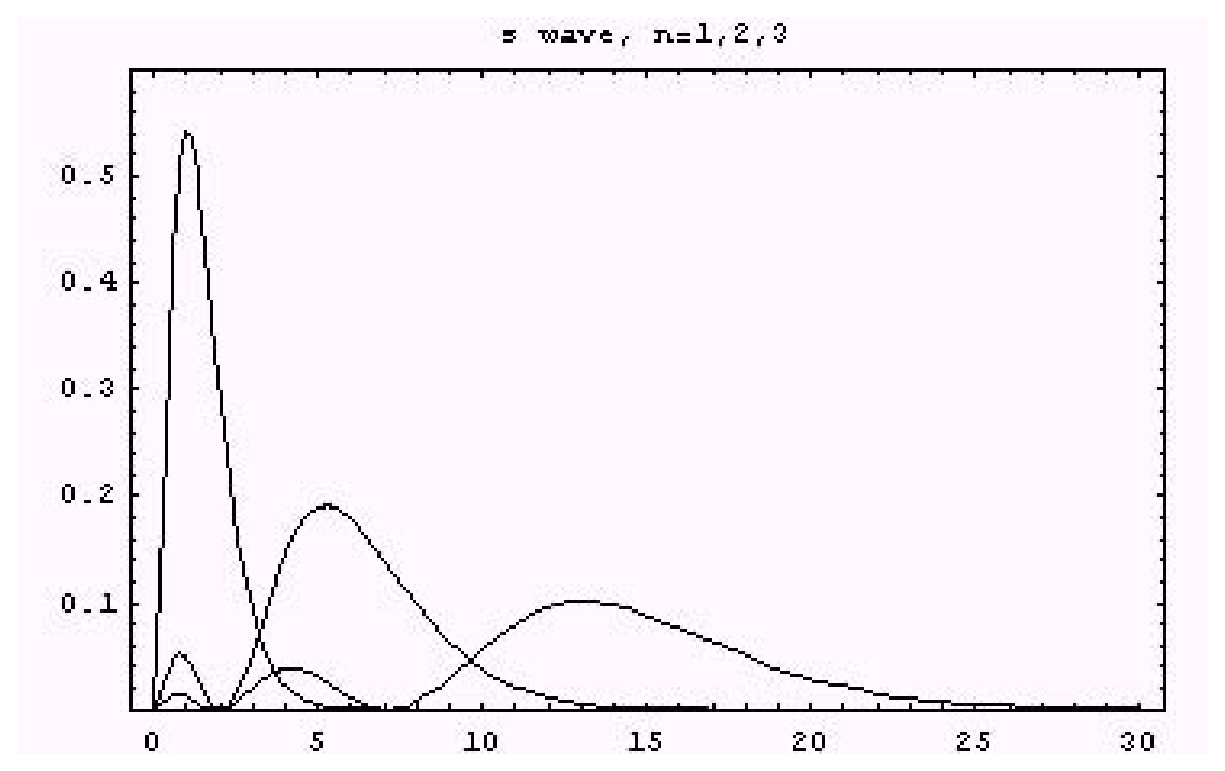
\includegraphics[clip,width=8cm]{HydrogenAtom/15-1.ps}
\caption{径向概率分布:s波,$n=1,2,3$}
\end{center}
\end{figure}

\begin{figure}[h]
\begin{center}
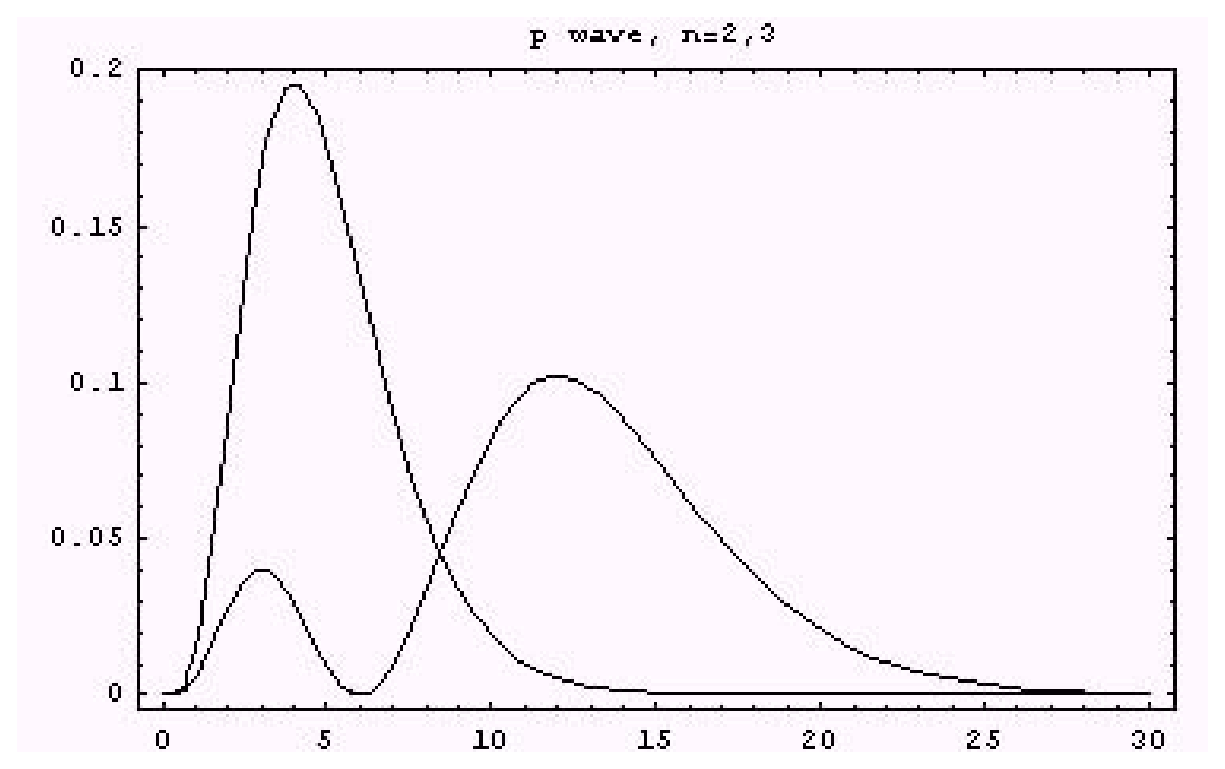
\includegraphics[clip,width=8cm]{HydrogenAtom/15-2.ps}
\caption{径向概率分布:p波,$n=2,3$}
\end{center}
\end{figure}


概率密度随空间角度的变化:$w(\theta ,\varphi ) d \Omega = \left| {Y_{lm} } \right|^2 d\Omega  \propto \left| {P_l^m \left( {\cos \theta } \right)} \right|^2 d\Omega $, $d\Omega  = \sin \theta d\theta d\varphi $

\begin{figure}[h]
\begin{center}
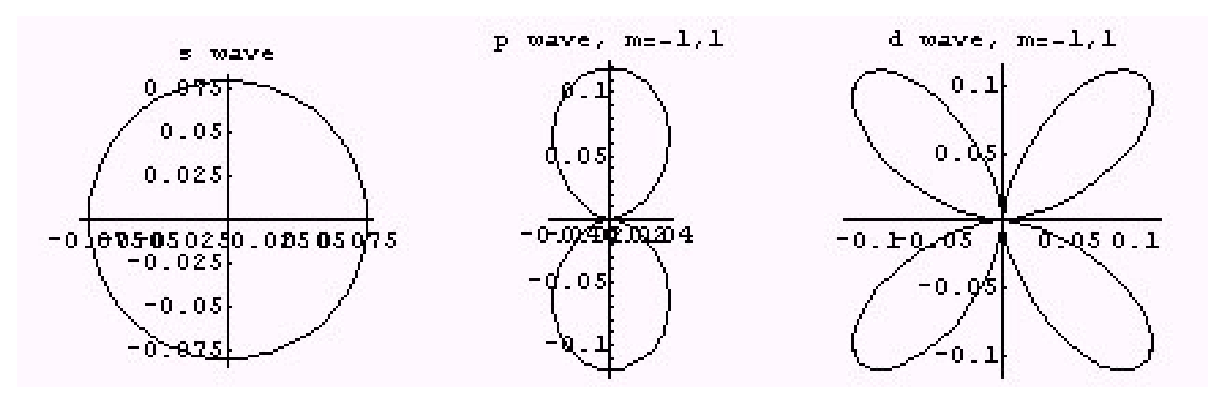
\includegraphics[clip,width=\textwidth]{HydrogenAtom/15-3.ps}
\caption{概率密度角度分布:1s波, 2p波($m = \pm 1$), 3d波($m = \pm 1$)}
\end{center}
\end{figure}

\subsubsection{氢原子光谱}

国际单位制下:$V(r) =  - \frac{{e^2 }}{{4\pi \varepsilon _0 r}}$, $\Rightarrow$
$E_n  =  - \frac{{me^4 }}{{2\hbar ^2 \left( {4\pi \varepsilon _0 } \right)^2 }}\frac{1}{{n^2 }} =  - \frac{{mc^2 }}{2}\left( {\frac{{e^2 }}{{4\pi \varepsilon _0 \hbar c}}} \right)^2 \frac{1}{{n^2 }}$

即:$E_n  =  - \frac{1}{2}m\left( {\alpha c} \right)^2 \frac{1}{{n^2 }}$, 精细结构常数:$\frac{{e^2 }}{{4\pi \varepsilon _0 \hbar c}} \equiv \alpha  \simeq \frac{1}{{137}}$

$h\nu  = E_n  - E_{n'} $

所以:$\tilde \nu  = \frac{1}{\lambda } = \frac{\nu }{c} = \frac{1}{{2hc}}m\left( {\alpha c} \right)^2 \left( {\frac{1}{{n^2 }} - \frac{1}{{n'^2 }}} \right)$,即里德堡公式。

里德堡常数为:$R_H  = \frac{1}{{2hc}}m\left( {\alpha c} \right)^2 $



\subsubsection{氢原子中的电流}

\begin{figure}[h]
\begin{center}
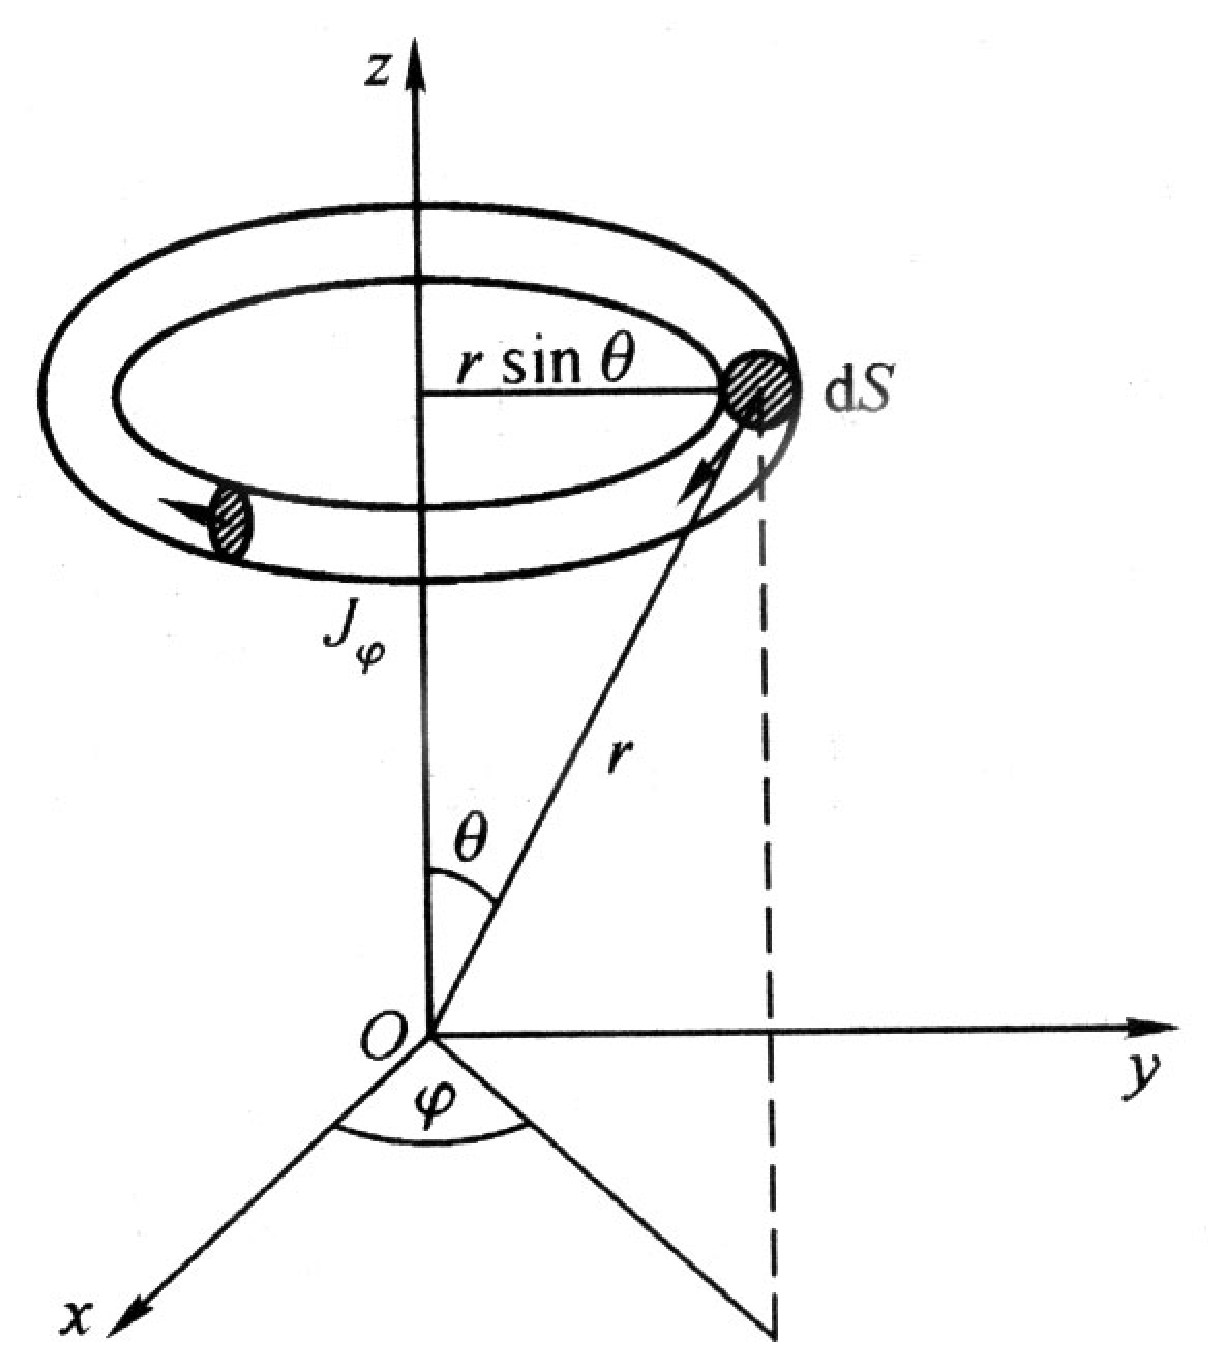
\includegraphics[clip,width=7cm]{HydrogenAtom/15-4.ps}
\caption{氢原子中的电流元}
\end{center}
\end{figure}

粒子流密度:$J =  - \frac{{i\hbar }}{{2\mu }}\left[ {\psi ^* \left( {\nabla \psi } \right) - \left( {\nabla \psi ^* } \right)\psi } \right]$

$\psi _{nlm} \left( {r,\theta ,\varphi } \right) = R_{nl} \left( r \right)Y_{lm} \left( {\theta ,\varphi } \right) = R_{nl} \left( r \right)\Theta _{l,m} \left( \theta  \right)\Phi _m \left( \varphi  \right) = R_{nl} \left( r \right)\Theta _{l,m} \left( \theta  \right)e^{im\varphi } $

球坐标下:$\nabla \psi  = \vec e_r \frac{{\partial \psi }}{{\partial r}} + \vec e_\theta  \frac{1}{r}\frac{{\partial \psi }}{{\partial \theta }} + \vec e_\varphi  \frac{1}{{r\sin \theta }}\frac{{\partial \psi }}{{\partial \varphi }}$

流密度的分量可写为:

$J_r^{(nlm)}  =  - \frac{{i\hbar }}{{2\mu }}\left( {\psi _{nlm}^* \frac{\partial }{{\partial r}}\psi _{nlm}  - \psi _{nlm} \frac{\partial }{{\partial r}}\psi _{nlm}^* } \right)\vec e_r  = 0$

$J_\theta ^{(nlm)}  =  - \frac{{i\hbar }}{{2\mu }}\left( {\psi _{nlm}^* \frac{1}{r}\frac{\partial }{{\partial \theta }}\psi _{nlm}  - \psi _{nlm} \frac{1}{r}\frac{\partial }{{\partial \theta }}\psi _{nlm}^* } \right)\vec e_\theta   = 0$

只有$J_\varphi ^{(nlm)}$,环绕$z$轴方向的几率流可能不为0:

\begin{eqnarray*}
J_\varphi ^{(nlm)}  & = &  - \frac{{i\hbar }}{{2\mu }}\left( {\psi _{nlm}^* \frac{1}{{r\sin \theta }}\frac{\partial }{{\partial \varphi }}\psi _{nlm}  - \psi _{nlm} \frac{1}{{r\sin \theta }}\frac{\partial }{{\partial \varphi }}\psi _{nlm}^* } \right)\vec e_\varphi   \\
{} & = & \frac{{m\hbar }}{{\mu r\sin \theta }}\left| {\psi _{nlm} } \right|^2 \vec e_\varphi
\end{eqnarray*}

相应电流密度在球坐标系中的分量是:

\begin{eqnarray*}
J_{er} & = & J_{e\theta }  = 0 \\
J_{e\varphi } & = &  - eJ_\varphi   =  - \frac{{me\hbar }}{{\mu r\sin \theta }}\left| {\psi _{nlm} } \right|^2 , m = 0, \pm 1, \pm 2,..., \pm l
\end{eqnarray*}

\subsubsection{氢原子中的磁矩}

氢原子中电流密度仅在$\vec e_\varphi  $方向上有贡献,$\vec e_\varphi  $方向电流元:$dI = J_{e\varphi } d\sigma $
$\vec e_\varphi  $方向电流元组成以$r\sin \theta $为半径的电流环,相应磁矩元为:

\index{Magnetic moment: 磁矩}

\begin{equation}
dM_z  = dIS\vec n = J_{e\varphi } d\sigma \left( {\pi r^2 \sin ^2 \theta } \right)
\end{equation}

总磁矩为:

\begin{eqnarray*}
M_z & = & \int {dM_z }  = \int {J_{e\varphi } d\sigma \left( {\pi r^2 \sin ^2 \theta } \right)}  = \int { - \frac{{me\hbar }}{{\mu r\sin \theta }}\left| {\psi _{nlm} } \right|^2 d\sigma \left( {\pi r^2 \sin ^2 \theta } \right)}  \\
{} & = &  - \int {\frac{{me\hbar }}{{2\mu }}} \left( {2\pi r\sin \theta } \right)\left| {\psi _{nlm} } \right|^2 d\sigma  =  - \frac{{me\hbar }}{{2\mu }}\int {2\pi r\sin \theta \left| {\psi _{nlm} } \right|^2 d\sigma }
\end{eqnarray*}

考虑到波函数$\psi _{nlm} $是归一化的:

\begin{eqnarray*}
\int {\left| {\psi _{nlm} } \right|^2 d\tau } & = & \int {\left| {\psi _{nlm} } \right|^2 r^2 \sin \theta d\theta d\varphi dr}  = \int {\left| {\psi _{nlm} } \right|^2 \left( {2\pi r\sin \theta } \right)rd\theta dr} \\
{} & = & \int {2\pi r\sin \theta \left| {\psi _{nlm} } \right|^2 d\sigma }  = 1
\end{eqnarray*}

所以:

\begin{equation}\label{15-15}
M_z  =  - \frac{{me\hbar }}{{2\mu }} =  - m\mu _B, m = 0, \pm 1, \pm 2,..., \pm l
\end{equation}


$\mu _B  = \frac{{e\hbar }}{{2\mu }}$称为玻尔磁子(Bohr
magneton);$M_z$是电子在库仑势场中运动引起,也叫轨道磁矩;$m$表示轨道磁矩的取值,因此$m$也叫磁量子数;

\index{Bohr magneton: 玻尔磁子}

角动量算符$z$分量本征值:

\begin{equation*}
l_z  = m\hbar; m = 0, \pm 1, \pm 2,..., \pm l
\end{equation*}

定义电子轨道运动的回转磁比率为:

\begin{equation}
\frac{{M_z }}{{l_z }} =  - \frac{{me\hbar }}{{2\mu m\hbar }} =  - \frac{e}{{2\mu }} =  - g_L \frac{e}{{2\mu }}
\label{gyro_magnetic_ration}
\end{equation}

其中:$g_L  = 1$(称为:朗德$g$因子),电子的自旋角动量与内禀磁矩关系与此不同,$g$因子的值为2。

由公式(\ref{gyro_magnetic_ration}),轨道磁矩\footnote{关于``磁矩'', 请阅读杨福家《原子物理学》第202页。}可用算符表示为:

\begin{equation}\label{15-16}
\widehat M_z  =  - g_L \frac{e}{{2\mu }}\widehat L_z
\end{equation}


